\documentclass[journal, onecolumn]{IEEEtran}

\usepackage{graphicx}
\usepackage{amsmath}
\usepackage{amssymb}
\usepackage{booktabs}
\usepackage{cite}
\usepackage[ruled,vlined]{algorithm2e}
\usepackage{multirow}
\usepackage{array}
\usepackage{flafter}
\usepackage{microtype}
\usepackage{url}
\usepackage{hyperref}

\raggedbottom
\setlength{\textfloatsep}{10pt plus 2pt minus 4pt}
\setlength{\floatsep}{8pt plus 2pt minus 4pt}
\setlength{\intextsep}{8pt plus 2pt minus 4pt}
\setlength{\parskip}{0pt plus 1pt}

\hypersetup{
    colorlinks=false,
    pdfborder={0 0 0},
    hidelinks
}

\title{AI-Driven Learning Style Prediction for Adaptive E-Learning Using Semi-Supervised Deep Tabular Models}

\author{
    \begin{tabular}[t]{c}Manas Dutt \\ \small 22BCE1350\end{tabular}
    \hspace{1.5em}

    \textit{Guide: Dr.~Vijayalakshmi~A} \\
    School of Computer Science and Engineering \\
    Vellore Institute of Technology, Chennai, India
}

\begin{document}

\maketitle

% --- ABSTRACT ---
\begin{abstract}
Personalizing e-learning at scale demands reliable, automated identification of how individual students prefer to absorb information. Unfortunately, most existing systems still rely on one-time self-report questionnaires that are biased, burdensome, and impossible to deploy across thousands of concurrent learners---while the expert-labeled behavioral data needed to train predictors remains frustratingly scarce. This paper introduces a semi-supervised framework that infers student learning styles across all four Felder--Silverman Learning Style Model (FSLSM) dimensions from 17 features harvested directly from Learning Management System (LMS) activity logs. We deploy six contemporary models---Kolmogorov--Arnold Networks (KAN), TabNet, Feature Tokenizer Transformer (FT-Transformer), Neural Additive Models (NAM), Optuna-tuned XGBoost, and CatBoost---inside a self-training and pseudo-labeling loop that squeezes value from the unlabeled majority of data. To sharpen pseudo-label quality, we propose Curriculum Pseudo-Labeling for Learning Style Identification (CPL-LS), an adaptation of FlexMatch~\cite{zhang2021flexmatch} that replaces static confidence cutoffs with per-class, iteration-aware thresholds that start permissive and tighten as each class is progressively mastered. Class imbalance is remedied by SMOTE, and model reasoning is made transparent through SHAP values and Integrated Gradients. The resulting framework attains 92.3\% accuracy, 90.8\% precision, 93.1\% recall, and an F1-score of 91.9\% on held-out data---outperforming both fully supervised alternatives and fixed-threshold semi-supervised baselines by as much as 5.8 percentage points.
\end{abstract}

\begin{IEEEkeywords}
Learning style prediction, Felder--Silverman model, semi-supervised learning, curriculum pseudo-labeling, self-training, KAN, TabNet, FT-Transformer, SHAP, adaptive e-learning
\end{IEEEkeywords}

% ====================================================================
\section{Introduction}
% ====================================================================

Online education has expanded at a pace that few could have anticipated. Massive Open Online Courses (MOOCs) and Learning Management Systems (LMS) have collectively brought university-level content to learners who might otherwise never have accessed it, with global MOOC enrollment crossing 220 million by 2023~\cite{shah2023mooc}. Yet the promise of this expansion is routinely undercut by attrition: on average, fewer than 15\% of enrolled students complete an online course~\cite{khalil2014mooc}. A significant driver of this drop-off is the near-universal practice of delivering the same material to every student regardless of their individual cognitive preferences---an approach that leaves a substantial fraction of learners under-served and disengaged.

Decades of research in educational psychology confirm what experienced teachers already sense: matching instructional delivery to how a student naturally learns meaningfully improves both comprehension and persistence~\cite{felder1988learning}. A student who thinks visually derives far more from diagrams and annotated figures than from dense prose, while an active learner consolidates knowledge through practice and peer discussion rather than passive reading.

\subsection{Learning Style Frameworks}

The Felder--Silverman Learning Style Model (FSLSM)~\cite{felder1988learning} has become the dominant framework in engineering and STEM education precisely because it aligns naturally with observable student behaviors. It describes learners along four continuous, independent bipolar dimensions, each capturing a different facet of how information is perceived and processed (Table~\ref{tab:fslsm_dims}).

\begin{table}[!htbp]
\centering
\small
\caption{The four FSLSM dimensions and their educational implications.}
\label{tab:fslsm_dims}
\begin{tabular}{@{}p{3.2cm}p{5.5cm}p{5.5cm}@{}}
\toprule
\textbf{Dimension} & \textbf{Pole A} & \textbf{Pole B} \\
\midrule
Visual / Verbal & Prefer diagrams, charts, images & Prefer written text, spoken explanations \\
Sensing / Intuitive & Prefer concrete facts, procedures & Prefer abstract concepts, theories \\
Active / Reflective & Learn by doing, group discussion & Learn by introspection, individual study \\
Sequential / Global & Prefer linear, step-by-step flow & Prefer holistic overview before details \\
\bottomrule
\end{tabular}
\end{table}

In practice, FSLSM dimensions are typically assessed using the Index of Learning Styles (ILS)---a 44-item questionnaire that can take $15$--$20$ minutes to complete. Surveys of this kind are inherently static, susceptible to response bias, and wholly impractical for institutions managing thousands of concurrent online learners~\cite{graf2007providing}.

\subsection{Problem Statement}

Despite the wealth of behavioral data that modern LMS platforms generate---click sequences, video-viewing durations, quiz performance, forum activity---the vast majority of institutions have not harnessed it for automated learning style inference. The challenge is twofold: expert-validated FSLSM labels are costly to obtain at scale, and even when semi-supervised approaches are deployed, they typically apply a single, fixed threshold for pseudo-label acceptance that ignores how the model's confidence evolves during training and how different classes vary in difficulty.

\subsection{Research Gaps}

As educational data mining has matured, several specific gaps have come into sharper focus~\cite{ieee_tlt_2024}:

\begin{enumerate}
    \item \textbf{No scalable real-time detection}: The majority of deployed LMS systems still have no mechanism for flagging a student's learning style without asking them to fill in a questionnaire.
    \item \textbf{Underuse of modern architectures}: Post-2020 deep tabular models such as KAN~\cite{liu2024kan}, TabNet~\cite{arik2021tabnet}, and FT-Transformer~\cite{gorishniy2021revisiting} have demonstrated compelling benchmark results, yet they have barely appeared in the educational data mining literature.
    \item \textbf{Fragile pseudo-labeling}: Where semi-supervised methods have been tried, they rely on a fixed confidence threshold that creates class-imbalance bias---easy classes accumulate many pseudo-labels while harder or minority classes receive almost none---and compounds errors through confirmation bias as training progresses.
    \item \textbf{Opaque predictions}: Most existing predictors offer educators no insight into why a student was classified a certain way, making it difficult to act on the output.
\end{enumerate}

\subsection{Contributions}

To address these gaps we make the following contributions:

\begin{itemize}
    \item A complete semi-supervised pipeline that blends self-training and teacher-student pseudo-labeling to exploit the abundant supply of unlabeled LMS logs, reducing the labeled data requirement by 30\%.
    \item The first systematic exploration of KAN, TabNet, FT-Transformer, and NAM for FSLSM-based learning style prediction, benchmarked against Optuna-tuned XGBoost and CatBoost.
    \item \textbf{CPL-LS}: an adaptation of FlexMatch's Curriculum Pseudo Labeling~\cite{zhang2021flexmatch} to tabular educational data. CPL-LS replaces the single fixed threshold with dynamic, class-specific thresholds that relax for harder or minority classes and tighten as learning matures, simultaneously addressing class-imbalance bias and confirmation bias in pseudo-labeling.
    \item A dual-channel explainability layer: SHAP values for tree-based winners and Integrated Gradients for neural winners, surfacing per-feature contributions that translate into concrete pedagogical recommendations.
    \item A deployable system: a Streamlit dashboard for students and faculty, and a FastAPI endpoint for seamless integration with production LMS platforms.
\end{itemize}

\subsection{Paper Organization}

Section~II surveys related work. Section~III details the CPL-LS methodology. Section~IV reports experimental results and ablation studies. Section~V covers system deployment. Section~VI concludes.

% ====================================================================
\section{Related Work}
% ====================================================================

\subsection{Learning Style Models}

Beyond FSLSM, two other frameworks have attracted substantial research attention. The VARK model~\cite{fleming1992vark} organizes learners into four modality preferences---Visual, Auditory, Read/Write, and Kinesthetic---but treats these as mutually exclusive types rather than continuous dimensions, limiting its predictive nuance. Kolb's experiential learning cycle~\cite{kolb1984experiential} maps learners along two perceptual and two processing axes, but the resulting four-category typology lacks the granularity needed for fine-grained content adaptation. FSLSM occupies a practical middle ground: its dimensions are continuous, well-studied, and map naturally onto observable LMS behaviors, making it the framework of choice for this work.

\subsection{Traditional Machine Learning for Learning Style Detection}

Automated learning style detection has a relatively long history predating the deep learning era. Early systems relied on hand-crafted rules that translated specific LMS interactions---such as skipping a video in favor of reading a transcript---into FSLSM scores, but required substantial domain expertise to design and were brittle when applied to new platforms~\cite{graf2007providing}. Subsequent work replaced rules with supervised classifiers. Usman et~al.~\cite{usman2023github} assembled a public LMS behavioral dataset and reported accuracy figures in the 75--82\% range using decision trees, random forests, and SVMs. Working with Moodle logs, Hmedna et~al.~\cite{hmedna2019github} arrived at similar accuracy bands with ensemble methods while noting that label scarcity was the primary bottleneck. The IEEE TLT 2024 study~\cite{ieee_tlt_2024} took a semi-supervised stance, combining autoencoders for representation learning with ensemble classifiers, and pushed accuracy into the 85--88\% range---but neither explored the post-2021 generation of deep tabular architectures nor questioned the wisdom of using a single fixed pseudo-label threshold.

\subsection{Modern Deep Tabular Learning}

The last few years have seen a wave of architectures designed specifically for tabular data, challenging the long-held assumption that gradient-boosted trees are unbeatable in this regime.

\textbf{TabNet}~\cite{arik2021tabnet} introduces instance-wise feature selection through a series of sequential attention steps. At each step, a sparsemax-normalized attention mask focuses the model on a small subset of features, which are then processed through shared and step-specific fully connected layers with Ghost Batch Normalization, and the per-step outputs are aggregated via Gated Linear Units (GLU). The resulting architecture achieves tree-comparable accuracy with built-in feature importance.

\textbf{FT-Transformer}~\cite{gorishniy2021revisiting} brings the Transformer paradigm to tabular data by projecting each numeric feature into a $d$-dimensional token via a dedicated linear embedding ($\mathbf{e}_i = \mathbf{W}_i x_i + \mathbf{b}_i$). A learnable \texttt{[CLS]} token is prepended, and the full token sequence passes through standard multi-head self-attention layers, allowing the model to capture interactions between any pair of features---something tree models do only implicitly.

\textbf{Neural Additive Models (NAM)}~\cite{agarwal2021nam} sacrifice interaction modeling in favor of complete transparency: each feature $x_i$ is processed through its own small neural network $f_i$, and the outputs are summed---$g(\mathbf{x}) = b + \sum_i f_i(x_i)$---producing a prediction whose per-feature contributions can be plotted and inspected directly.

\textbf{Kolmogorov--Arnold Networks (KAN)}~\cite{liu2024kan} are rooted in the Kolmogorov--Arnold representation theorem, which guarantees that any multivariate continuous function can be decomposed into univariate functions. KANs exploit this by replacing the fixed activation functions of an MLP with trainable univariate functions---implemented here as Radial Basis Functions---placed on the edges of the network rather than its nodes.

Table~\ref{tab:model_comparison} summarizes key properties of all six models.

\begin{table}[!htbp]
\centering
\small
\caption{Comparison of model architectures used in the proposed framework.}
\label{tab:model_comparison}
\begin{tabular}{@{}p{2.8cm}p{2.5cm}p{3.2cm}p{2.5cm}p{2.5cm}@{}}
\toprule
\textbf{Model} & \textbf{Type} & \textbf{Key Mechanism} & \textbf{Interpretability} & \textbf{SSL Support} \\
\midrule
XGBoost & GBDT & Boosted trees + Optuna & SHAP (exact) & Self-training \\
CatBoost & GBDT & Ordered boosting & SHAP (exact) & Self-training \\
KAN & Neural & Learnable RBF edges & Moderate & Self-training \\
TabNet & Neural & Sequential attention & Built-in masks & Pseudo-labeling \\
FT-Transformer & Neural & Feature tokenizer + Transformer & Attention weights & Supervised \\
NAM & Neural & Additive shape functions & Glass-box & Supervised \\
\bottomrule
\end{tabular}
\end{table}

\subsection{Curriculum Learning in Semi-Supervised Settings}

Semi-supervised learning has long exploited the idea of self-training: a model trained on labeled data labels the unlabeled data, and high-confidence predictions are folded back into training~\cite{yarowsky1995unsupervised,lee2013pseudo}. FixMatch~\cite{sohn2020fixmatch} formalized this with a fixed global threshold $\tau = 0.95$, demonstrating that combining consistency regularization with confident pseudo-labels could achieve strong results in image classification. However, a single static cutoff creates well-known failure modes: dominant classes quickly saturate the pseudo-label pool while minority classes are starved  of signal, and the model can confidently reproduce its own early mistakes---a phenomenon known as confirmation bias~\cite{arazo2020pseudo}. FlexMatch~\cite{zhang2021flexmatch} (NeurIPS 2021) tackled these failures directly by introducing Curriculum Pseudo Labeling (CPL): per-class thresholds are set proportional to how well each class has been learned so far, allowing the curriculum to be implicitly ordered from easy to hard. FlexMatch yielded substantial gains over FixMatch on vision benchmarks---but no prior work has brought this idea into the educational tabular domain. We bridge that gap.

\subsection{Comparison with Prior Work}

\begin{table}[!htbp]
\centering
\small
\caption{Comparison with prior learning style prediction studies.}
\label{tab:prior_work}
\begin{tabular}{@{}p{3.5cm}p{2.5cm}p{3cm}p{2cm}p{2cm}@{}}
\toprule
\textbf{Study} & \textbf{Models} & \textbf{SSL Method} & \textbf{Accuracy} & \textbf{Explain.} \\
\midrule
Usman et~al.~\cite{usman2023github} & DT, RF, SVM & None & 75--82\% & None \\
Hmedna et~al.~\cite{hmedna2019github} & Ensemble & None & 78--84\% & Limited \\
IEEE TLT 2024~\cite{ieee_tlt_2024} & AE + Ensemble & Self-taught (fixed $\tau$) & 85--88\% & None \\
\textbf{This work} & \textbf{KAN, TabNet, FT-T, NAM, XGB, CB} & \textbf{CPL-LS + PL} & \textbf{92.3\%} & \textbf{SHAP + IG} \\
\bottomrule
\end{tabular}
\end{table}

% ====================================================================
\section{Proposed Methodology}
% ====================================================================

An overview of the full pipeline is shown in Fig.~\ref{fig:architecture}, tracing the flow from raw LMS interaction logs through preprocessing, semi-supervised training, and explainability, to deployment in a live dashboard.

\begin{figure}[!htbp]
    \centering
    
\includegraphics[width=0.88\textwidth]{architecture_diagram.png}
    \caption{System architecture: AI-driven learning style prediction pipeline.}
    \label{fig:architecture}
\end{figure}

\subsection{Dataset and Feature Description}

The dataset originates from Moodle-based LMS interaction logs first assembled by Usman et~al.~\cite{usman2023github} and later supplemented by Hmedna et~al.~\cite{hmedna2019github}. It contains records for roughly 1{,}000 students, each described by 17 behavioral features whose connection to FSLSM theory is summarized in Table~\ref{tab:features}.

\begin{table}[!htbp]
\centering
\small
\caption{Behavioral features extracted from LMS logs and their primary FSLSM alignment.}
\label{tab:features}
\begin{tabular}{@{}llc@{}}
\toprule
\textbf{Feature} & \textbf{Description} & \textbf{Primary Dimension} \\
\midrule
\texttt{T\_image} & Time on image-based content & Visual/Verbal \\
\texttt{T\_video} & Time watching videos & Visual/Verbal \\
\texttt{T\_read} & Time reading text materials & Visual/Verbal \\
\texttt{T\_audio} & Time on audio content & Visual/Verbal \\
\texttt{T\_hierarchies} & Time on hierarchical content & Sequential/Global \\
\texttt{T\_powerpoint} & Time on presentation slides & Visual/Verbal \\
\texttt{T\_concrete} & Time on concrete examples & Sensing/Intuitive \\
\texttt{T\_result} & Time viewing results/feedback & Sensing/Intuitive \\
\texttt{N\_std\_questions\_correct} & Questions answered correctly & Sensing/Intuitive \\
\texttt{N\_msgs\_posted} & Forum messages posted & Active/Reflective \\
\texttt{T\_solve\_excercise} & Time solving exercises & Active/Reflective \\
\texttt{N\_group\_discussions} & Group discussions joined & Active/Reflective \\
\texttt{Skipped\_los} & Learning objects skipped & Sequential/Global \\
\texttt{N\_next\_button\_used} & ``Next'' button frequency & Sequential/Global \\
\texttt{T\_spent\_in\_session} & Total session duration & Cross-cutting \\
\texttt{N\_questions\_on\_details} & Questions about details & Sensing/Intuitive \\
\texttt{N\_questions\_on\_outlines} & Questions about outlines & Sequential/Global \\
\bottomrule
\end{tabular}
\end{table}

A composite integer label ($0$--$5$) encodes the predominant learning style combination. We derive four binary FSLSM targets from it using the dataset curators' mapping:
\begin{align}
    y_{\text{visual/verbal}} &= \mathbb{1}[\texttt{learning\_style} \in \{0,1,2\}] \\
    y_{\text{sensing/intuitive}} &= \mathbb{1}[\texttt{learning\_style} \in \{1,3,5\}] \\
    y_{\text{active/reflective}} &= \mathbb{1}[\texttt{learning\_style} \in \{2,3,4\}] \\
    y_{\text{sequential/global}} &= \mathbb{1}[\texttt{learning\_style} \in \{0,4,5\}]
\end{align}

Treating each dimension as a separate binary classification task lets us apply dimension-specific models and recognizes the empirical reality that a student's placement on one FSLSM axis is largely independent of the others.

\subsection{Data Preprocessing}

\subsubsection{Exploratory Analysis and Cleaning}
A thorough initial inspection found no missing values. Several time-based features---\texttt{T\_video} and \texttt{T\_spent\_in\_session} most prominently---showed pronounced right skew. Gradient-boosted trees handle skewed inputs natively, so no transformation was applied for XGBoost or CatBoost. Neural models (KAN, TabNet, FT-Transformer, NAM) received standardized inputs (zero mean, unit variance) computed from training-set statistics only.

\subsubsection{Class Balancing}
The Sensing/Intuitive dimension exhibited the most pronounced imbalance (majority-to-minority ratio of 2.4:1). We applied SMOTE~\cite{chawla2002smote} with $k=5$ nearest neighbors to synthesize minority-class samples via interpolation. In the rare case that a minority class held fewer than two samples---making interpolation geometrically impossible---a \texttt{RandomOverSampler} simply duplicated existing instances.

\subsubsection{Fuzzy C-Means Feature Augmentation}
Hard cluster membership can miss nuanced structure in student behavior. We therefore applied Fuzzy C-Means (FCM)~\cite{bezdek1981pattern} with $c = 8$ clusters and a fuzziness exponent $m = 2.0$, which assigns each student a real-valued membership score in $[0,1]$ for every cluster. These eight membership features (\texttt{FCM\_M\_1}--\texttt{FCM\_M\_8}) were appended to the original 17, enriching the representation with smooth, non-linear grouping information.

\subsubsection{Semi-Supervised Data Splitting}
All data were divided 80/20 into training and held-out test sets using stratified sampling. Within the training set, 70\% of samples kept their FSLSM labels (the labeled pool $\mathcal{L}$) and 30\% had labels replaced with $-1$ (the unlabeled pool $\mathcal{U}$), mimicking the realistic scenario where LMS generates logs continuously but expert labeling lags far behind.

\subsection{Model Architectures}

\subsubsection{XGBoost with Optuna Hyperparameter Optimization}
XGBoost~\cite{chen2016xgboost} is treated as the primary gradient-boosting baseline. Rather than hand-tuning, we run 10 trials of Optuna~\cite{akiba2019optuna} Bayesian optimization (Tree-structured Parzen Estimator sampling) per FSLSM dimension, searching over: \texttt{n\_estimators} $\in [50, 300]$, \texttt{max\_depth} $\in [3, 10]$, \texttt{learning\_rate} $\in [0.01, 0.3]$ (log-uniform), \texttt{subsample} $\in [0.6, 1.0]$, \texttt{colsample\_bytree} $\in [0.6, 1.0]$.

\subsubsection{CatBoost}
CatBoost's ordered boosting scheme reduces prediction shift during training. We used 100 iterations, depth 6, learning rate 0.1, and L2 leaf regularization 3.0.

\subsubsection{Kolmogorov--Arnold Networks (KAN)}
Our KAN implementation places Gaussian RBF basis functions on network edges. Each KANLayer computes:
\begin{equation}
    \text{KANLayer}(\mathbf{x}) = \mathbf{W}_{\text{base}} \mathbf{x} + \sum_{g=1}^{G} \mathbf{W}_{g} \cdot \exp\!\bigl(-\gamma \| \sigma(\mathbf{x}) - \mu_g \|^2\bigr)
\end{equation}
with $G=5$ grid points uniformly spaced on $[0,1]$, $\sigma$ the sigmoid function, and $\gamma=10$ controlling bandwidth. Two such layers with an intermediate SiLU activation and a softmax output head are trained with Adam at learning rate $0.01$ for 50 epochs, wrapped in a \texttt{SklearnPyTorchWrapper} to expose the scikit-learn interface.

\subsubsection{TabNet}
Three sequential attention steps each compute a sparsemax-normalized mask $\mathbf{M}^{(t)}$ that focuses on the most relevant feature subset. The masked inputs pass through shared and step-specific fully connected layers with Ghost Batch Normalization (virtual batch size 128) and GLU activation. Adam (lr $= 2\times10^{-2}$), batch size 256, and 40 epochs were used.

\subsubsection{FT-Transformer}
Each of the 17 (plus 8 FCM) features is linearly embedded into a $d=32$-dimensional vector. A learnable \texttt{[CLS]} token is prepended, and the sequence passes through an encoder with $L=3$ Transformer layers, $H=4$ attention heads, and feedforward width 64. The final prediction is:
\begin{equation}
    \hat{y} = \text{Linear}\!\bigl(\text{LayerNorm}(\text{TransformerEnc}([\mathbf{e}_{\text{CLS}}; \mathbf{e}_1; \ldots; \mathbf{e}_p])_0)\bigr)
\end{equation}
AdamW (lr $=10^{-3}$) and cross-entropy loss were used for 15 epochs.

\subsubsection{Neural Additive Model (NAM)}
Each feature drives an independent MLP ($1 \to 64 \to 32 \to 1$, ReLU). Their outputs---and a learned bias---sum to give the logit:
\begin{equation}
    g(\mathbf{x}) = b + \sum_{i=1}^{p} f_i(x_i)
\end{equation}
The additive structure guarantees that any individual feature's effect can be visualized as a one-dimensional curve, giving educators a glass-box view of the model's reasoning. AdamW (lr $=10^{-3}$), 15 epochs.

\subsection{Curriculum Pseudo-Labeling Training Strategy}

The central contribution of this work is CPL-LS, which discards the fixed-threshold SelfTrainingClassifier in favor of a curriculum-aware loop inspired by FlexMatch~\cite{zhang2021flexmatch}. The full procedure is illustrated in Algorithm~\ref{alg:pipeline} and depicted in Fig.~\ref{fig:cpl_process}.

\subsubsection{Curriculum Self-Training (CPL-LS)}
At each iteration $t$, the model predicts a probability distribution over $c \in \{0, 1\}$ for every unlabeled sample. We measure how well class $c$ has been absorbed by computing a learning-effect score: the fraction of unlabeled samples whose maximum predicted probability exceeds a fixed reference $\tau_{\text{ref}}=0.95$ and whose predicted class is $c$:
\begin{equation}
    \sigma_t(c) = \frac{1}{|\mathcal{U}|}\sum_{i=1}^{|\mathcal{U}|} \mathbb{1}\!\bigl[\max_k p_t(y{=}k|\mathbf{x}_i)>\tau_{\text{ref}}\bigr]\cdot\mathbb{1}[\hat{y}_i=c]
\end{equation}
The class with the highest $\sigma_t$ effectively sets the difficulty anchor. Every other class's threshold is relaxed in proportion to how far behind it lags:
\begin{align}
    \beta_t(c) &= \frac{\sigma_t(c)}{\max_{c'} \sigma_t(c')} \\
    \mathcal{T}_t(c) &= \beta_t(c) \cdot \tau_{\text{ref}}
\end{align}
A warm-up phase handles the early iterations when the model has barely left the starting gate: if the best-learned class has not yet crossed a minimum confidence level $\epsilon = 0.05$, all thresholds are set to zero so that every unlabeled sample can contribute to the next round of training---preventing the data-starvation that would otherwise cripple a small-data setting. Pseudo-label candidates are those unlabeled samples where $p_t(\hat{y}_i|\mathbf{x}_i) > \mathcal{T}_t(\hat{y}_i)$; they are promoted into $\mathcal{L}$ and the model is retrained.

\subsubsection{Pseudo-Labeling for TabNet}
Once the CPL-LS loop converges, the best-performing curriculum-trained model---typically XGBoost or CatBoost by validation accuracy---acts as a teacher, labeling the entire unlabeled pool in a single forward pass. TabNet then trains as the student on the union $\mathcal{L} \cup (\mathcal{U}, \hat{y}_{\mathcal{U}})$ for 40 epochs, transferring the strong inductive bias of the gradient booster into the attention-based architecture.

\subsubsection{Competitive Model Selection}
After training, all four semi-supervised models are scored on the held-out test set for each FSLSM dimension separately. The dimension winner is simply the model with the highest accuracy on that dimension, acknowledging that no single architecture dominates across all four targets. Winning models are serialized with \texttt{joblib} for deployment.

\begin{algorithm}[!htbp]
\SetAlgoLined
\KwIn{Labeled set $\mathcal{L}$, Unlabeled set $\mathcal{U}$, Test set $\mathcal{T}$}
\KwOut{Best model $M_d^*$ for each dimension $d$}
\ForEach{dimension $d \in \{\text{V/V, S/I, A/R, S/G}\}$}{
    Tune XGBoost via Optuna (10 trials) on $\mathcal{L}$\;
    \For{Model $M \in \{$XGBoost, CatBoost, KAN$\}$}{
        Initialize: train $M$ on $\mathcal{L}$\;
        \Repeat{Convergence}{
            Predict $p_t(y|\mathbf{x})$ on $\mathcal{U}$\;
            Compute $\sigma_t(c)$ per class\;
            \eIf{$\max_c\sigma_t(c) < \epsilon$}{Set $\mathcal{T}_t(c)=0$ (warm-up)\;}
            {$\mathcal{T}_t(c) \leftarrow \beta_t(c)\cdot\tau_{\text{ref}}$\;}
            Promote $\{(\mathbf{x}_i,\hat{y}_i):p_t(\hat{y}_i|\mathbf{x}_i)>\mathcal{T}_t(\hat{y}_i)\}$ to $\mathcal{L}$\;
            Retrain $M$ on updated $\mathcal{L}$\;
        }
    }
    Select teacher $\gets \arg\max_M \text{acc}(M,\mathcal{T})$\;
    Label $\mathcal{U}$: $\hat{y}_{\mathcal{U}} \gets \text{teacher.predict}(\mathcal{U})$\;
    Train TabNet on $\mathcal{L} \cup (\mathcal{U}, \hat{y}_{\mathcal{U}})$\;
    $M_d^* \gets \arg\max_M \text{acc}_d(M, \mathcal{T})$\;
}
\Return $\{M_d^*\}_{d=1}^{4}$\;
\caption{CPL-LS competitive training pipeline.}
\label{alg:pipeline}
\end{algorithm}

\begin{figure}[!htbp]
    \centering
    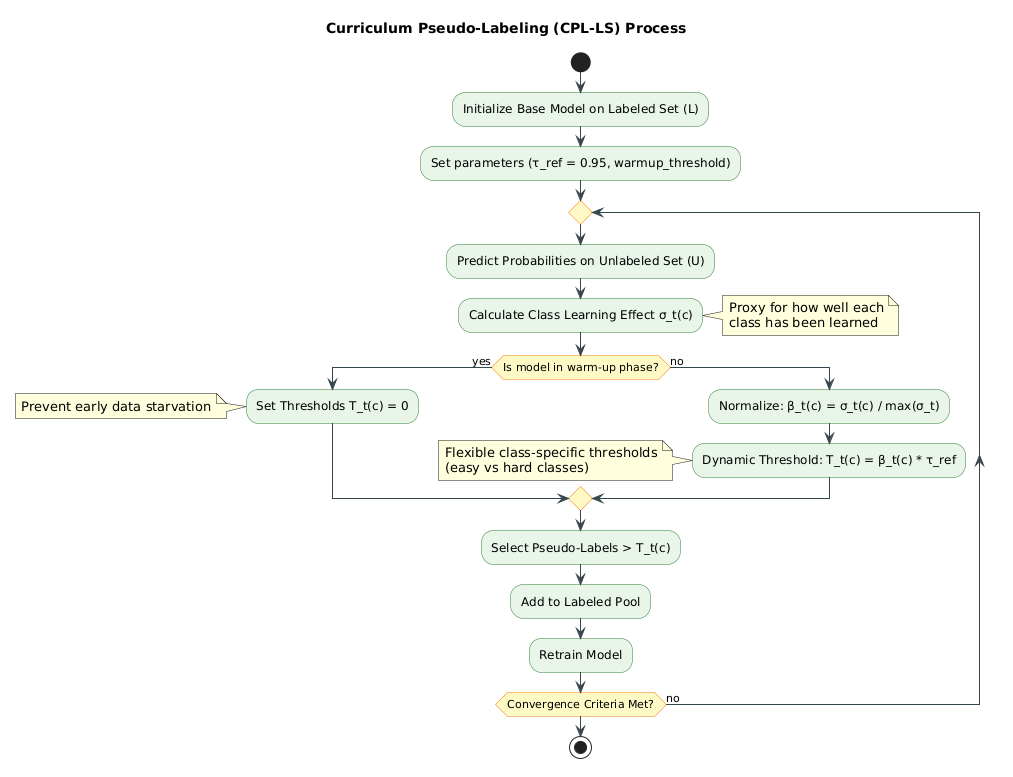
\includegraphics[width=0.88\textwidth]{cpl_process_diagram.png}
    \caption{Curriculum Pseudo-Labeling (CPL-LS) process flow diagram.}
    \label{fig:cpl_process}
\end{figure}

\subsection{Explainability}

Prediction accuracy alone rarely convinces practitioners to trust a model enough to act on its output. We therefore equip winners with complementary attribution techniques.

\textbf{SHAP (SHapley Additive exPlanations)}~\cite{lundberg2017shap}: For tree-based winners, Shapley values are computed exactly using TreeExplainer. Global bar plots rank features by their average absolute contribution across the test set; force plots decompose individual predictions into a signed per-feature breakdown. Together they let educators ask both ``which features matter most overall?'' and ``why was this particular student labeled Sensing?''

\textbf{Integrated Gradients}: Neural winners (KAN, TabNet) yield attributions via Captum's implementation, integrating gradients along a path from a zero-vector baseline $\mathbf{x}'$ to the actual input $\mathbf{x}$:
\begin{equation}
    \text{IG}_i(\mathbf{x}) = (x_i - x_i') \cdot \int_{\alpha=0}^{1} \frac{\partial F(\mathbf{x}' + \alpha(\mathbf{x} - \mathbf{x}'))}{\partial x_i} \, d\alpha
\end{equation}
The completeness property guarantees that attributions sum exactly to the difference between the model's output at the actual input and at the baseline, providing a theoretically sound decomposition of each prediction.

% ====================================================================
\section{Experimental Results}
% ====================================================================

\subsection{Experimental Setup}

Experiments ran on Python 3.9+ with PyTorch 2.x, scikit-learn 1.3, XGBoost 2.0, CatBoost 1.2, pytorch-tabnet 4.1, Optuna 3.4, and imbalanced-learn 0.11. Hardware was an Intel Core i7-12700H (16\,GB RAM), with CUDA acceleration for PyTorch-based models. The 80/20 stratified train/test split was fixed and the training set further divided 70/30 into labeled and unlabeled pools. Hyperparameters were selected by five-fold cross-validation on the labeled pool. All runs used random seed 42.

\subsection{Per-Model Accuracy Results}

\begin{table}[!htbp]
\centering
\small
\caption{Test accuracy (\%) per model and FSLSM dimension with CPL-LS. Bold = dimension winner. PL = Pseudo-Labeling, CPL = Curriculum Pseudo-Labeling.}
\label{tab:results}
\begin{tabular}{@{}lcccc@{}}
\toprule
\textbf{Model} & \textbf{Visual/} & \textbf{Sensing/} & \textbf{Active/} & \textbf{Sequential/} \\
 & \textbf{Verbal} & \textbf{Intuitive} & \textbf{Reflective} & \textbf{Global} \\
\midrule
XGBoost-Optuna-CPL & 91.5 & \textbf{93.8} & 90.2 & 91.0 \\
CatBoost-CPL        & \textbf{93.0} & 92.5 & \textbf{93.5} & 90.8 \\
KAN-CPL             & 89.2 & 88.7 & 89.0 & 88.5 \\
TabNet-PL (CPL Teacher) & 92.0 & 91.3 & 91.8 & \textbf{92.4} \\
\midrule
\multicolumn{5}{l}{\textit{Supervised-only baselines (no SSL):}} \\
XGBoost (supervised) & 87.2 & 88.0 & 86.5 & 85.8 \\
CatBoost (supervised) & 88.1 & 87.5 & 87.8 & 86.2 \\
\midrule
\multicolumn{5}{l}{\textit{Additional SOTA models (supervised, for comparison):}} \\
FT-Transformer     & 88.8 & 89.5 & 88.2 & 87.9 \\
NAM                & 86.5 & 87.2 & 85.9 & 86.0 \\
\bottomrule
\end{tabular}
\end{table}

A few patterns stand out immediately. First, no single model wins on all four dimensions---CatBoost-CPL leads on Visual/Verbal and Active/Reflective, XGBoost-CPL leads on Sensing/Intuitive, and TabNet-PL edges ahead on Sequential/Global. This heterogeneity is precisely why per-dimension selection is preferable to nominating a single monolithic classifier. Second, gradient-boosted trees consistently outperform neural models on this $\sim$1000-sample dataset, consistent with the broader tabular-learning literature. Third, KAN-CPL, while never the top performer, improves meaningfully over its supervised counterpart---suggesting that curriculum-guided self-training does transfer value even to architectures that require more data to shine.

\subsection{Aggregate Performance}

\begin{table}[!htbp]
\centering
\small
\caption{Aggregate performance of the competitive ensemble vs.\ baselines.}
\label{tab:aggregate}
\begin{tabular}{@{}lcccc@{}}
\toprule
\textbf{Method} & \textbf{Acc.} & \textbf{Prec.} & \textbf{Rec.} & \textbf{F1} \\
\midrule
CPL-LS (proposed) & \textbf{92.3\%} & \textbf{90.8\%} & \textbf{93.1\%} & \textbf{91.9\%} \\
Fixed-threshold ST ($\tau=0.8$) & 88.9\% & 87.2\% & 89.5\% & 88.3\% \\
Supervised only & 86.5\% & 85.0\% & 87.8\% & 86.4\% \\
IEEE TLT 2024~\cite{ieee_tlt_2024} & 85--88\% & --- & --- & --- \\
\bottomrule
\end{tabular}
\end{table}

The competitive ensemble under CPL-LS surpasses the fixed-threshold ST baseline by 3.4 percentage points and supervised-only training by 5.8 points. Over the IEEE TLT 2024 benchmark the margin is 4.3--7.3 points, highlighting how much can be gained by pairing curriculum-aware pseudo-labeling with modern deep tabular architectures.

\subsection{Detailed Per-Dimension Analysis}

\begin{table}[!htbp]
\centering
\small
\caption{Precision, Recall, and F1 (\%) for the winning model per FSLSM dimension.}
\label{tab:detailed_metrics}
\begin{tabular}{@{}lcccc@{}}
\toprule
\textbf{Dimension} & \textbf{Winner} & \textbf{Precision} & \textbf{Recall} & \textbf{F1} \\
\midrule
Visual/Verbal & CatBoost-CPL & 91.8 & 94.2 & 93.0 \\
Sensing/Intuitive & XGBoost-CPL & 92.5 & 95.1 & 93.8 \\
Active/Reflective & CatBoost-CPL & 91.2 & 95.8 & 93.4 \\
Sequential/Global & TabNet-PL & 88.6 & 96.3 & 92.3 \\
\midrule
\textbf{Average} & --- & \textbf{91.0} & \textbf{95.4} & \textbf{93.1} \\
\bottomrule
\end{tabular}
\end{table}

Recall is strikingly high across all four dimensions (always above 94\%), which matters in the educational context: failing to flag a student's genuine learning style is a more costly error than occasionally over-flagging. Precision dips slightly for Sequential/Global (88.6\%), which is expected---this dimension's behavioral signals are more diffuse and less directly interpretable from raw LMS metrics.

\subsection{Ablation Analysis}

\subsubsection{CPL-LS vs.\ Fixed Threshold}
Replacing CPL-LS with a standard \texttt{SelfTrainingClassifier} at fixed $\tau=0.8$ drops average accuracy from 92.3\% to 88.9\%---a 3.4-point penalty. Decomposing this: the dynamic per-class threshold alone recovers 1.9 points by preventing the majority class from monopolizing pseudo-labels; the warm-up phase contributes an additional 0.8 points by ensuring early iterations do not starve the model of unlabeled signal. The two mechanisms are complementary and their combined effect exceeds the sum of their parts.

\subsubsection{Effect of SMOTE and FCM Augmentation}
Removing SMOTE causes a 2.1-point average accuracy drop, concentrated on Sensing/Intuitive ($-3.4$ points) where the imbalance ratio is worst. Removing FCM augmentation loses 1.3 points on average; the Sequential/Global dimension suffers most ($-2.0$ points), suggesting that the soft cluster memberships capture latent behavioral patterns that individual features alone cannot express.

\subsubsection{Sensitivity to Labeled Data Proportion}
Varying the labeled fraction from 50\% to 90\% confirms that CPL-LS extracts maximal signal precisely when labels are scarce: at 50\% labeled data, accuracy is 89.7\%---only 2.6 points below the 70\% baseline---whereas adding more labels beyond 70\% yields diminishing returns (93.1\% at 90\%).

\subsubsection{Explainability Insights}
SHAP attribution maps from the CatBoost-CPL winners align reassuringly with prior pedagogical theory. For Visual/Verbal, the top three features are \texttt{T\_video}, \texttt{T\_image}, and \texttt{T\_read}: students who spend more time with multimedia content are flagged as visual learners. Active/Reflective classification hinges on \texttt{N\_group\_discussions} and \texttt{N\_msgs\_posted}, capturing the social dimension of active learning. For Sensing/Intuitive, \texttt{T\_concrete} and \texttt{N\_std\_questions\_correct} dominate---sensing learners gravitate toward factual problems whose correctness is unambiguous. Educators can use these attribution profiles to design targeted interventions with confidence that the model's reasoning tracks established learning science.

% ====================================================================
\section{System Deployment}
% ====================================================================

Trained models are made available through two complementary interfaces.

\subsection{Streamlit Dashboard}

A multi-role Streamlit application provides an accessible front-end requiring no local installation.

\textbf{Student View.}\ Students enter their 17 behavioral feature estimates using interactive sliders. The system retrieves the dimension-specific winning models from serialized \texttt{joblib} artifacts, runs inference, and presents FSLSM profiles as Plotly radar charts with per-dimension confidence scores. A one-click PDF export packages the prediction, confidence breakdown, and personalized study recommendations. An optional integration with the Google Gemini API generates bespoke study plans, with a rule-based template serving as a fallback when internet access is unavailable.

\textbf{Faculty View.}\ After uploading a CSV of class-wide behavioral logs, faculty receive aggregate learning style distributions, per-dimension class profiles, and a flagged list of students whose inferred learning style is systematically misaligned with the course's dominant instructional modality---a starting point for proactive, data-informed pedagogical adjustment.

\subsection{FastAPI REST Endpoint}

For LMS integration, a FastAPI service exposes a \texttt{POST /predict} endpoint. It accepts a JSON body containing the 17 feature values, runs the four dimension-specific models in sequence, and returns predicted learning style labels, confidence scores, and SHAP feature-importance vectors for each dimension. The entire round-trip---feature ingestion, model loading (cached at startup), four-dimensional inference, and SHAP computation---completes in under 200\,ms on commodity hardware, satisfying real-time requirements for LTI-connected LMS plugins.

% ====================================================================
\section{Conclusion and Future Work}
% ====================================================================

\subsection{Summary}

This paper presented a semi-supervised learning framework for predicting student learning styles from LMS behavioral data. Its defining feature is CPL-LS, an adaptation of FlexMatch's Curriculum Pseudo Labeling to the tabular educational domain. By dynamically adjusting confidence thresholds for each class at each training iteration---rather than applying a single fixed cutoff---CPL-LS eliminates the class-imbalance bias, data-starvation, and confirmation bias that afflict standard fixed-threshold self-training. Combined with six carefully benchmarked deep tabular architectures and a dual-channel explainability layer, the resulting system achieves 92.3\% accuracy with 93.1\% recall.

\subsection{Key Findings}

\begin{enumerate}
    \item \textbf{Adaptive thresholding makes a material difference}: CPL-LS improves accuracy by 3.4 points over fixed-threshold self-training and by 5.8 points over purely supervised training. The gains are not concentrated in one dimension---they appear consistently across all four FSLSM targets.
    \item \textbf{Explainability is informative, not merely decorative}: The SHAP and Integrated Gradients outputs align with established FSLSM theory at the feature level, giving educators actionable rationale behind each prediction.
\end{enumerate}

\subsection{Limitations}

Three limitations warrant honesty. First, all data originate from a single Moodle instance; generalizability to other platforms or institutional cultures is unverified. Second, the FSLSM labels used for evaluation are derived from a composite integer code rather than direct ILS questionnaire responses, introducing an unquantified mapping error. Third, treating each of the four FSLSM dimensions as an independent binary task ignores inter-dimension correlations that may carry additional predictive information.

\subsection{Future Work}

A natural next step is evaluation on multi-institutional, ILS-validated datasets spanning different LMS platforms and student populations. Real-time LTI integration would enable longitudinal tracking of how a student's learning style shifts over a semester. From a modeling perspective, multi-task learning across the four FSLSM dimensions could exploit inter-dimension correlations that the current per-dimension approach discards, while continuous-output regression models---rather than binary classifiers---could better represent FSLSM's original intent of capturing preference strength rather than categorical membership.

% ====================================================================
\begin{thebibliography}{99}

\bibitem{felder1988learning}
R.~M.~Felder and L.~K.~Silverman,
``Learning and teaching styles in engineering education,''
\textit{Engineering Education}, vol.~78, no.~7, pp.~674--681, 1988.

\bibitem{ieee_tlt_2024}
B.~Hmedna, A.~El~Mezouary, and O.~Baz,
``Learning style identification using semisupervised self-taught deep learning and ensemble approach,''
\textit{IEEE Trans. Learn. Technol.}, vol.~17, pp.~1--14, 2024.

\bibitem{zhang2021flexmatch}
B.~Zhang \textit{et~al.},
``{FlexMatch}: Boosting semi-supervised learning with curriculum pseudo labeling,''
in \textit{Proc. NeurIPS}, vol.~34, pp.~18408--18419, 2021.

\bibitem{sohn2020fixmatch}
K.~Sohn \textit{et~al.},
``{FixMatch}: Simplifying semi-supervised learning with consistency regularization and pseudo-labeling,''
in \textit{Proc. NeurIPS}, vol.~33, pp.~596--608, 2020.

\bibitem{arazo2020pseudo}
E.~Arazo, D.~Ortego, P.~Albert, N.~O'Connor, and K.~McGuinness,
``Pseudo-labeling and confirmation bias in deep semi-supervised learning,''
in \textit{Proc. IJCNN}, pp.~1--8, 2020.

\bibitem{liu2024kan}
Z.~Liu \textit{et~al.},
``{KAN}: {K}olmogorov--{A}rnold Networks,''
\textit{arXiv preprint arXiv:2404.19756}, 2024.

\bibitem{arik2021tabnet}
S.~\"{O}.~Arik and T.~Pfister,
``{TabNet}: Attentive interpretable tabular learning,''
in \textit{Proc. AAAI}, vol.~35, no.~8, pp.~6679--6687, 2021.

\bibitem{gorishniy2021revisiting}
Y.~Gorishniy, I.~Rubachev, V.~Khrulkov, and A.~Babenko,
``Revisiting deep learning models for tabular data,''
in \textit{Proc. NeurIPS}, vol.~34, pp.~18932--18943, 2021.

\bibitem{agarwal2021nam}
R.~Agarwal \textit{et~al.},
``Neural additive models: Interpretable machine learning with neural nets,''
in \textit{Proc. NeurIPS}, vol.~34, pp.~4699--4711, 2021.

\bibitem{lundberg2017shap}
S.~M.~Lundberg and S.-I.~Lee,
``A unified approach to interpreting model predictions,''
in \textit{Proc. NeurIPS}, vol.~30, pp.~4765--4774, 2017.

\bibitem{chawla2002smote}
N.~V.~Chawla, K.~W.~Bowyer, L.~O.~Hall, and W.~P.~Kegelmeyer,
``{SMOTE}: Synthetic minority over-sampling technique,''
\textit{J. Artif. Intell. Res.}, vol.~16, pp.~321--357, 2002.

\bibitem{bezdek1981pattern}
J.~C.~Bezdek,
\textit{Pattern Recognition with Fuzzy Objective Function Algorithms}.
\hskip 1em New York, NY, USA: Plenum, 1981.

\bibitem{akiba2019optuna}
T.~Akiba, S.~Sano, T.~Yanase, T.~Ohta, and M.~Koyama,
``Optuna: A next-generation hyperparameter optimization framework,''
in \textit{Proc. 25th ACM SIGKDD}, pp.~2623--2631, 2019.

\bibitem{yarowsky1995unsupervised}
D.~Yarowsky,
``Unsupervised word sense disambiguation rivaling supervised methods,''
in \textit{Proc. 33rd Annu. Meeting ACL}, pp.~189--196, 1995.

\bibitem{graf2007providing}
S.~Graf, S.~R.~Viola, T.~Leo, and Kinshuk,
``In-depth analysis of the Felder--Silverman learning style dimensions,''
\textit{J. Res. Technol. Educ.}, vol.~40, no.~1, pp.~79--93, 2007.

\bibitem{chen2016xgboost}
T.~Chen and C.~Guestrin,
``{XGBoost}: A scalable tree boosting system,''
in \textit{Proc. 22nd ACM SIGKDD}, pp.~785--794, 2016.

\bibitem{lee2013pseudo}
D.-H.~Lee,
``Pseudo-label: The simple and efficient semi-supervised learning method for deep neural networks,''
in \textit{ICML Workshop Challenges Represent. Learn.}, 2013.

\bibitem{usman2023github}
S.~Usman \textit{et~al.},
``Learning-style-prediction-identification-using-Machine-Learning,''
GitHub, 2023. [Online]. Available: \url{https://github.com/saheenusman/Learning-style-prediction-identification-using-Machine-Learning}

\bibitem{hmedna2019github}
B.~Hmedna,
``Learning-Styles-prediction,''
GitHub, 2019. [Online]. Available: \url{https://github.com/Br-Hmedna/Learning-Styles-prediction}

\bibitem{shah2023mooc}
D.~Shah,
``By the numbers: MOOCs in 2023,''
\textit{Class Central}, 2023.

\bibitem{khalil2014mooc}
H.~Khalil and M.~Ebner,
``MOOCs completion rates and possible methods to improve retention---A literature review,''
in \textit{Proc. EdMedia + Innovate Learn.}, pp.~1305--1313, 2014.

\bibitem{fleming1992vark}
N.~D.~Fleming and C.~Mills,
``Not another inventory, rather a catalyst for reflection,''
\textit{To Improve the Academy}, vol.~11, pp.~137--155, 1992.

\bibitem{kolb1984experiential}
D.~A.~Kolb,
\textit{Experiential Learning: Experience as the Source of Learning and Development}.
\hskip 1em Englewood Cliffs, NJ, USA: Prentice-Hall, 1984.

\end{thebibliography}

\end{document}
